\usepackage{graphicx}


\chapter{Introduction - Project Context}
\label{ch:introduction}
\pagestyle{headings}

\section{Project context}
\label{sec:introduction-context}

\subsection{General Context}
\label{subsec:introduciton-general-context}

In the last century, because of advances in technology and medicine, the average lifespan has increased to a global \
average of 70.5 years, with and European average of about 80.2 years\
\footnote{According to https://en.wikipedia.org/wiki/List\_of\_countries\_by\_life\_expectancy}, with more details in \
\ref{table:lifeExpectancy}. \
This in turn has led to people taking better care for themselves at older ages. \
There are several ways to improve life quality and extend life expectancy. \
Most doctors agree that one of the most important ones is a correct diet.

\begin{table}[ht]
    \caption{Average Life Expectancy in Europe}
    \centering                          % tabel centrat
    \begin{tabular}{|c|c|c|}          % 3 coloane centrate
        \hline\hline                        % linie orizontala dubla
        Area & Male & Female \\ [0.5ex]   % inserare tabel
        %heading
        \hline                              % linie orizontal simpla
        Europe & 75 & 81 \\               % corpul tabelului
        Western Europe & 79 & 84  \\
        Southern Europe & 79 & 84 \\           % [1ex] adds vertical space
        Northern Europe & 79 & 83  \\
        Eastern Europe & 68 & 78 \\[1ex]
        \hline
    \end{tabular}
    \label{table:lifeExpectancy}
\end{table}

\subsection{Specific Context}
\label{subsec:introduction-specific-context}

As people get older, their biological functions begin to fail, and they start to experience health issues. \
According to \
the World Health Organization\footnote{http://www.who.int/news-room/fact-sheets/detail/mental-health-of-older-adults},\
an estimated 15\% of all adults over 60 suffer from some sort of mental disorder. \
Some of the most common are depression, anxiety and dementia. \
This can lead to either a lack or an increased appetite, either of which can lead to a chemical \
imbalance in the body, causing even more health problems. \
Another common issue among elder people is the degradation of \
senses. \
People tend to lose the sense of smell, taste, sight, which means they cannot be fully aware of what they eat.\
Without strict control, this can lead to people eating foods that may be harmful to them without even knowing (such as \
people having heart problems with too salty foods and not sensing it).


\subsection{Nutrients}
\label{subsec:introduction-nutrients}
There are a few nutrients that are very important to the organism, and we will present them briefly.

Proteins are one of these nutrients. \
For instance, hair and nails are mostly made of protein, along with muscular tissue. \
They are required to build enzymes, hormones and other chemicals found in the human body. \
For active people, theoretically there is no upper intake limit. \
However, out target group is make of elder people, and an important fact \
that needs to be taken into account is that proteins contain about 4 calories/100g. \
On the other hand, a lack of proteins \
can cause diarrhea, fatigue, loss of muscle mass, lethargy, reduced immunity and can ultimately lead to death.

Lipids are another important group of nutrients. \
They naturally occur in fats, monoglycerids, fat-soluble vitamins and others. \
They are mainly used to store energy, as part of the membrane that surrounds cells, as building blocks for \
several hormones and as components of the nervous system. \
Excess consumption of lipids can cause multiple cardio-vascular problems and obesity. \
Underconsumption can also lead to health issues.

Carbo-hydrates are also an important nutrient, as they are a source of energy. \
However, they are not essential to humans,as people can take most of their energy from proteins and fats. \
Excess consumption often leads to type 1 diabetes.

Another major group of important nutrients are minerals. \
Calcium is generally important for health, as it is being used by the nervous system, muscles, heart and bones. \
Over-consumption over a long period of time can lead to a higher risk of kidney stones, while lack if calcium in \
the body can lead to osteoporosis (thinning of bone tissue and decreased bone density).

Iron is another essential mineral. \
It is one of the components of hemoglobin, which is used by red blood cells to carry oxygen throughout the body. \
About two thirds of the iron in the human body is found in hemoglobins. \
Lack of iron can lead to fatigue, dizziness and lowered immunity. \
Excess iron can build up in organism, leading to diseases like liver cancer, cardiac arrhythmia, diabetes, \
Alzheimer's, bacterial and viral infections.

Sodium is another important mineral in health. \
It plays a part in muscle contraction and nerve impulse conduction. \
Lack sodium causes cellular functions and neural communication to stop. \
Excess iron builds up in blood vessels, causing over time high blood pressure, heart attack and stroke.

Another important group of nutrients is made of vitamins. \
Vitamin A is naturally occurs in many foods. \
It plays a part vision, immune system and reproduction. \
Lack of it can cause sight issues, while excess can lead to dizziness, headaches, coma or even death.

The B-vitamin family plays a part in turning food into energy and metabolizing fats. \
This family contains 8 vitamins (B1-B8). \
B6 is used in the digestive, immune, muscular, cardiovascular and nervous system.Lack of it can cause anemia, \
rashes or swollen tongue, depression, weak immune system and confusion.
Excess can cause nerve damage.

Vitamin C is required for normal growth and development. \
However, consuming more than 2000mg/day can lead to stomach upset and diarrhea. \
Lack of it can cause symptoms of deficiency, such as bleeding gums, anemia, weaker immune system, \
weight gain, painful or swollen joints.

Vitamin D is also important for good overall health. \
It plays a part in the function of muscles, lungs, heart, brain and immune system. \
It is required for the absorption of calcium. \
Lack of vitamin D over longer periods of time can lead to \
fragile bones in adults, colon cancer, prostate cancer, depression, heart diseases, weight gain and more. \
Excess can cause kidney stones, heart problems, confusion, nausea.


\subsection{Motivation}
\label{subsec:introduction-motivation}
Europe is dealing with an increasingly older population. \
Lifespan is continuously increasing and several European populations are dealing with major problems concerning \
demographic changes and the transition to a much older population structure.


\begin{figure}[ht]
    %\centering
    \label{fig:eurostat1}
    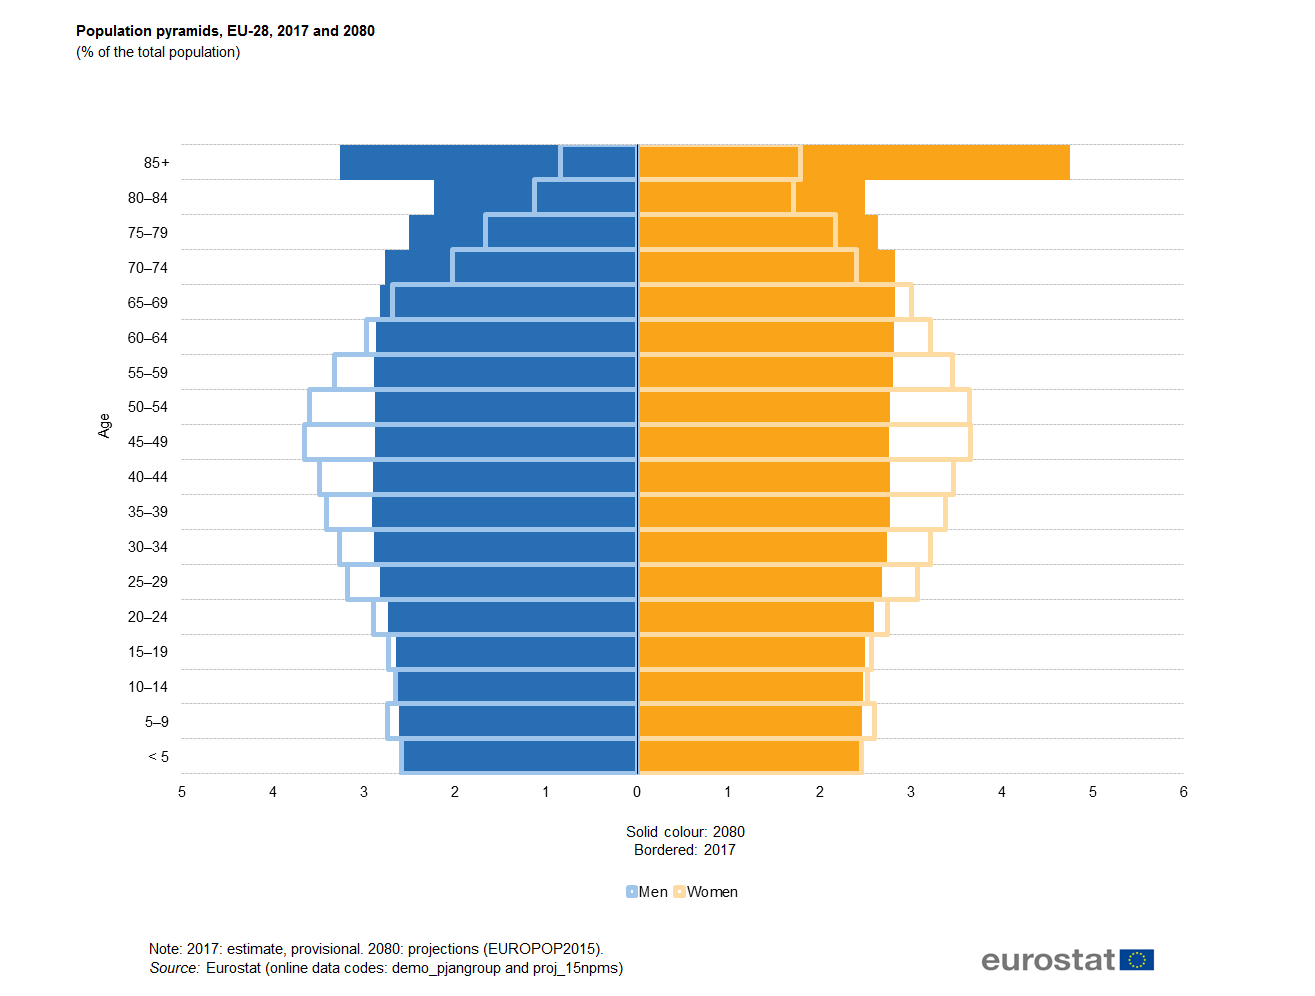
\includegraphics[width=15cm, height=60cm,keepaspectratio]{img/eurostat1.png}
    \caption{Population pyramid in 2080 compared to 2017, according to Eurostat}
\end{figure}

According to ~\cite{eurostat1}, as can be seen in figure \ref{fig:eurostat1}, current predictions estimate \
that the percentage of elder people will increase. \
Estimates put the number of people aged 65 years or more as approximately 29.1\% of \
the total population by 2080, compared to the current value of approximately 19.4\%.

Although it may seem that a longer life is a good thing, and indeed the advances in medicine and technology from \
the last century have granted us longer lives, an important issue remains the distinction between lifespan and the \
quality of life. \
According to a study made by the University of South Carolina between 1970 and 2010,
\footnote{https://news.usc.edu/98750/americans\-living\-longer\-with\-disability\-or\-health\-issues\-study\-shows/},\
although the total lifespan increased in this period, so did the time spent with a disability. \
This means that people need to pay more attention to living healthy. \
And in order to do that, people need to eat healthy first.
